\chapter{Concatemers detection on rolling circle DNA amplification of viral genome}\label{ch:concatemers}
\thispagestyle{empty}
\vspace*{\fill}
\epigraph{\emph{Another quote}}
{Son Nguyen}

\clearpage
%%%%%%%%%%%%%%%%%%%%%%%%%%%%%%%%%%%%%%%%%%%%%%%%

This chapter describes an additional application of MinION sequencing and computational methods involved to sequence viral genomes efficiently.
The study here will exploit the excessive length of single nanopore long reads to harbor multiple copies of a small-size whole genome DNA sequence. The sequence, given sufficient read depth, can be reconstructed from a high-resolution consensus calling. 
Even though this study do not emphasis on the real-time property of the device, it is straight-forward to adapt such pipeline using the developed modules.

\review{AWMC plasmid sequencing \& assembly: reasoning for the method...}
\section{Data description}
\paragraph{Viral samples}

\paragraph{Rolling circle DNA amplification}
\review{follow the link below}
%https://www.sigmaaldrich.com/technical-documents/protocols/biology/nucleic-acid-preparation/circular-dna-amplification-using-templiphi.html
\paragraph{MinION sequencing}
A rapid barcode sequencing has been conducted for 4 samples with barcode assignment as given in Table~\ref{tab:viral_samples}.
\begin{table}[!hpt]
\centering
\caption{Viral samples subjected to MinION barcoding sequencing}
\label{tab:viral_samples}
\begin{tabular}{|l|l|l|r|r|}
\hline
\textbf{Barcode} & \textbf{Sample} & \textbf{Description} & \textbf{Pass reads}  & \textbf{N50}    \\\hline
08                  & CaMV+              & \emph{Cauliflower mosaic} virus  &   14,385   &      6,707 \\\hline
09                  & BSMYV+             & \emph{Banana streak MY} virus    &   3,389   &   8,178   \\\hline        
10                  & BSMYV-             & \emph{Banana streak MY} virus, negative control     &   4,653   &  6,023   \\\hline
12                  & CaMV-              & \emph{Cauliflower mosaic} virus, negative control     &   9,942   &  4,919   \\\hline
\end{tabular}
\end{table}
\section{Bioinformatics analyses}
\subsection{Reference-based detection of concatemers}
Raw signal data from MinION were base-called and demultiplexed by \albacore{} version 2.1.0. This resulted in 4 DNA sequence files corresponding to 4 barcoded samples, only pass reads from those sequences were used for further analyses.

\paragraph{Work flow} Due to the application of rolling circle amplification, each long read is expected to contain more than one copy of the virus DNA, potentially sitting next to each other in a \emph{concatemer}. We create an in-house pipeline to detect and extract the \emph{monomer} sequences out of the reads to build their consensus as shown in Figure \ref{fig:concat_ref_workflow}.

\begin{figure}[ht]
\centerline{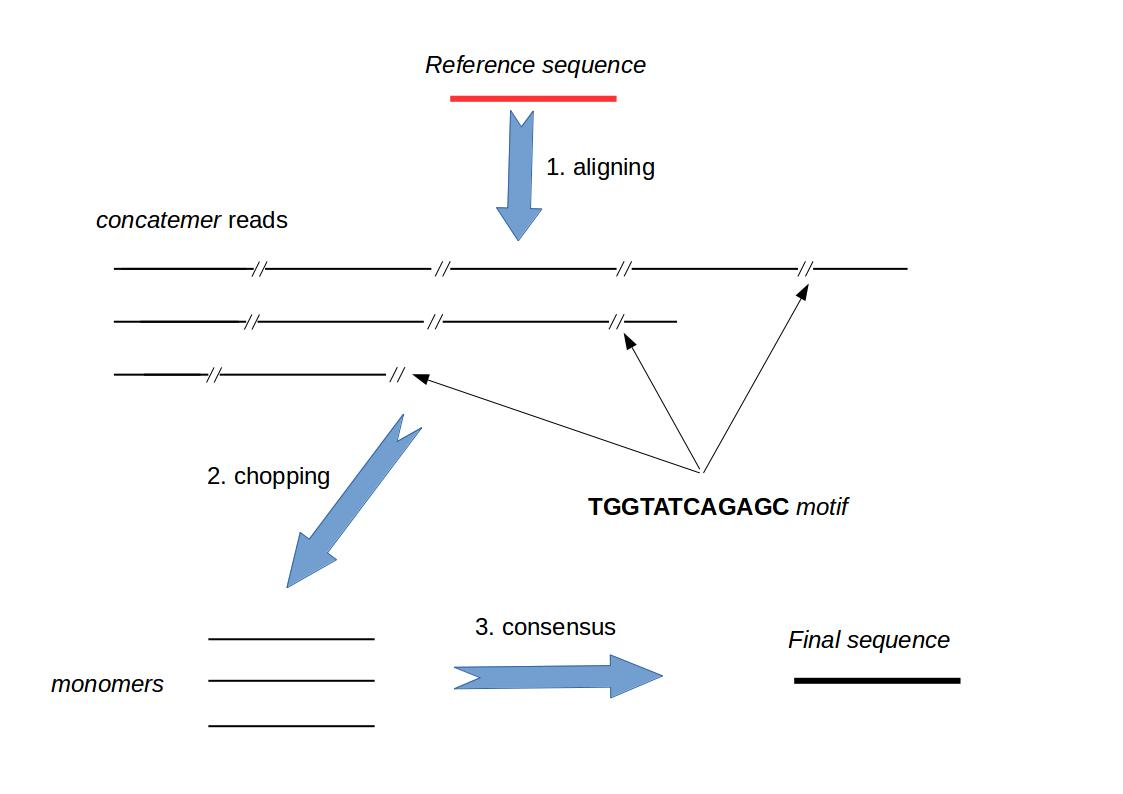
\includegraphics[width=0.9\textwidth]{images/concatemer.jpg}}
\caption{Pipeline to reconstruct viral genome sequences from MinION long reads.}
\label{fig:concat_ref_workflow}
\end{figure}

In more details, the pipeline is implemented by following the following steps: 
\begin{itemize}
\item[1.] align nanopore reads to the corresponding reference by \minimap{}~\cite{Li2016} version 2.11-r797 and keep only the ones covered $>80\%$ of the target; then induce locations of monomer on each reads based on the alignments.
\item[2.] for each monomer inferred, scanning for the nearest hit of 12nt motif \\\textbf{TGGTATCAGAGC}, then chop the read at those loci.
\item[3.] build consensus sequence on those monomers by \racon{}~\cite{Vaser2017racon} version 1.2.1.
\end{itemize}

\paragraph{Align to the reference}
Figures \ref{fig:bc08} and \ref{fig:bc09} show the read length histogram of only mapped reads from nanopore data of barcode 08 and 09 respectively. Two negative control samples (barcode 10 and 12) returned no hits when aligned to their corresponding reference thus not shown. As can be observed, CaMV virus (barcode 08) has richer sequencing data compared to BSMYV sample (barcode 09).
\begin{figure}[!ht]
\centering
\subfloat[Mapped reads from barcode 08\label{fig:bc08}]{
	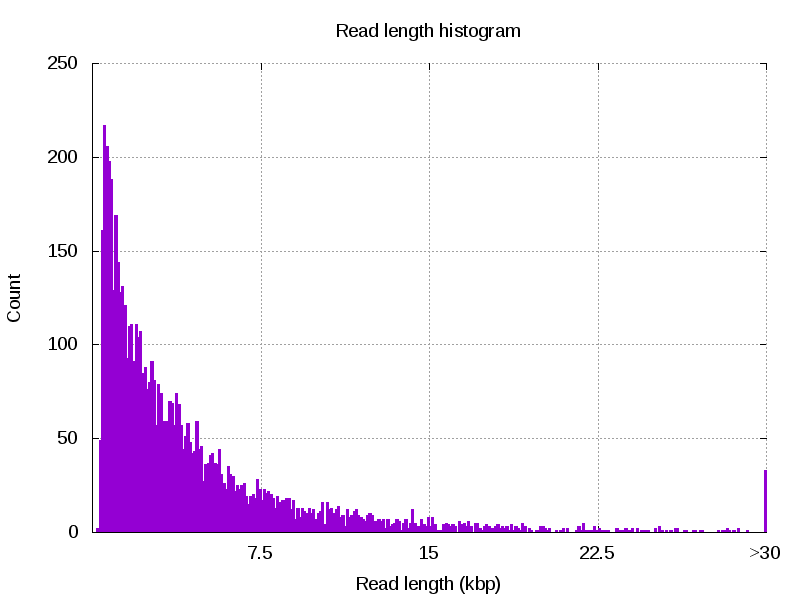
\includegraphics[width=.5\textwidth]{images/barcode08.png}
}
~
\subfloat[Mapped reads from barcode 09\label{fig:bc09}]{
	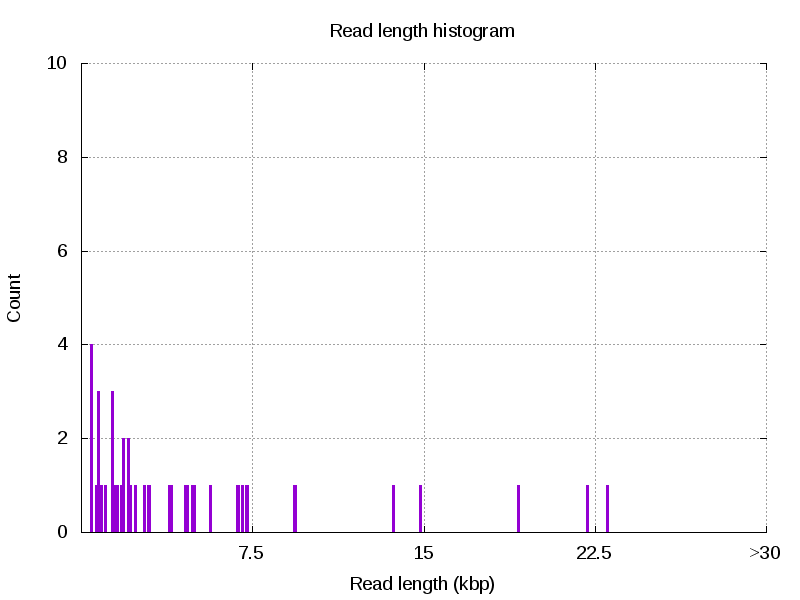
\includegraphics[width=.5\textwidth]{images/barcode09.png}
}
\caption{Mapped read length histogram of barcode 08 and 09.}
\label{fig:concat_map}
\end{figure}

\paragraph{Concatemer extraction}
Chart \ref{supp_fig:concat_count} presents the number of k-concatemers (concatemers with exact k monomers extracted) for each positive sample (barcode 08 and 09). 
The longest concatemer detected is a 7-concatemer of CaMV DNA sequence. 
There is also one 6-concatemer and one 4-concatemer from this sample. 
In addition, the numbers detected k-concatemers for \emph{Cauliflower mosaic} virus are greater than one for $k=3$ (2 reads) or $k=2$ (6 reads).
Monomer reads make up the most abundance group with 33 CaMV sequences and 5 BSMYV sequences.
There is no other concatemers detected for the latter sample.

The extraction step generated in total 68X and 5X monomers respectively for barcode 08 and 09. By using these monomer sequences, we can pile them up and call the consensus sequence from the erroneous nanopore data. The sequence coverage obtained plays a critical role for the accuracy of the result: for barcode 08, the consensus is $99.5\%$ identical to its reference while the figure is only $93.72\%$ in case of barcode 09. 

\subsection{Reference-free method}
Assuming no references are given, the duplication of a DNA sequence in a nanopore read can still be detectable by using self-alignment to study the repeat pattern.
An efficient approach to investigate periodic repeat patterns is to use auto-correlation function (ACF).
Similar signal processing based methods have been developed for fast biological sequence alignment and repeat detection \cite{Rockwood2005crosscorrelation,Ravi2007tandem}.
Here I present another application of this signal processing technique to detect the concatemers of the aforementioned viral sample using nanopore data. 
Tools are developed to work on both base-called and raw signal sequences.
In the following sections, only results for the longest 7-concatemer read (from barcoe 08 sample) are shown for demonstration purpose without loss of generalization.
\subsubsection{Auto-correlation function}
Given an infinite sequence of discrete signals $S=\ldots s_1 s_2 \ldots s_k \ldots$ where $S(i)=s_i$ , its ACF $f(n)$ is defined as the cross correlation to itself
\begin{equation}
 f(n)=\sum_{k}{s_k\ast s_{k-n}}   
 \label{eq:acf}
\end{equation}
where $\ast$ operator returns a similarity score when compare two operands, \EG{} complex conjugate for $s(i) \in \mathbb{C}$~\cite{Rockwood2005crosscorrelation}, and $n$ stands for the lag value. By increasing this value, we have a sliding dot product between the signal vector with itself which in expect give peaks when repeat parts of the sequence are overlapped as demonstrated in Figure~\ref{fig:concat_acf}. Note that for every signal sequence $S$, there is always a peak at $n=0$ as a result from self-overlapping. In addition, the ACF values are symmetric with regard to this center value.
\begin{figure}[ht]
\centerline{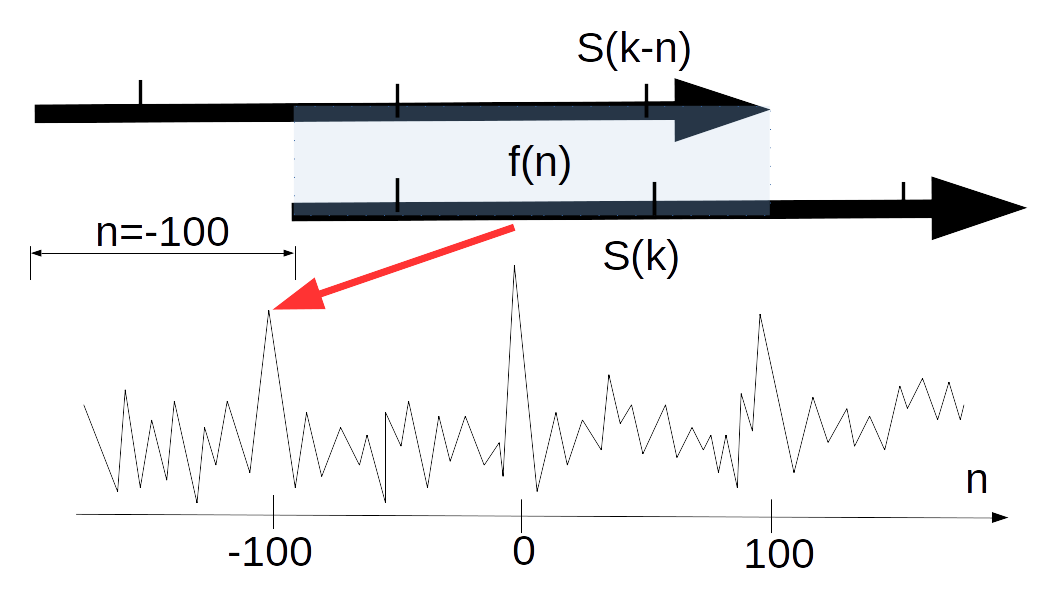
\includegraphics[width=0.7\textwidth]{images/acf.png}}
\caption[Example of ACF sliding dot product for a sequence with two repeats]{Example of ACF sliding dot product for a sequence with two repeats. The plots of ACF would return 3 peaks corresponding to $n=-100, n=0, n=100$.}
\label{fig:concat_acf}
\end{figure}

In fact, the signal sequence to process is definite: $S=\{s_i\}, i=1 \ldots L$ for sequence with length $L$. Out of range values are normally zero padded $s_j \equiv 0 \: \forall j \leq 0,j > L$ or duplicated so that $s_i \equiv s_{i+n \times L} \: \forall n \in \mathbb{Z}$. In this study, the former filling method is used.
\subsubsection{Concatemers detection on base-called sequence}
Given a DNA sequence, we have $S(i)=s_i \in \{A,C,G,T\} \: \forall i \in \mathbb{N}$. The letters are then equivalently numbered with positive values, \EG{} $\{1,2,3,4\}$ respectively.
Consequently, the $\ast$ operator from Equation~\ref{eq:acf} can be simply adapted to the Kronecker delta function
\[
s_i \ast s_j \equiv \delta_{s_i,s_j} = \left\{
\begin{array}{ll}
0     &  if \: s_i = s_j\\
1     &  if \: s_i \neq s_j
\end{array}
\right.
\]
As can be seen from Equation~\ref{eq:nkdf}, the ACF values are normalized by the overlap length to eliminate the position dependant property of the function which is helpful for picking peaks. Due to the error rate of MinION sequence data, a smoothing step is needed to average a window of nearby values. We set the window size equal to 10 for this scenario. 

Overall, for this case, we investigate the signal of the normalized Kronecker delta function (NKDF) as shown in Equation~\ref{eq:nkdf}
\begin{equation}
\label{eq:nkdf}
f(n) = \frac{\displaystyle \sum_{i=1}^{L}{\delta_{s_i,s_{i-n}}}}
            {\displaystyle L-|n|}
            , n \in (-L;L)
\end{equation}

\begin{figure}[!ht]
\centering
\subfloat[ACF for a random DNA sequence\label{fig:acf_random}]{
	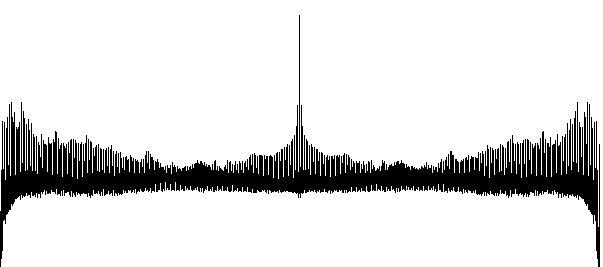
\includegraphics[width=.49\textwidth]{images/concatemer-random.png}
}
~
\subfloat[ACF for the 7-concatemer read\label{fig:acf_7cm}]{
	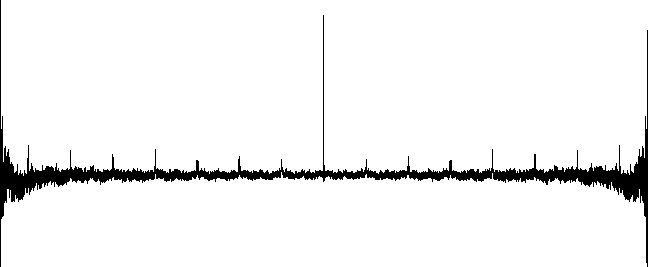
\includegraphics[width=.49\textwidth]{images/concatemer-7cm.png}
}
\caption{ACF values for a random read (\ref{fig:acf_random}) versus the 7-concatemer detected (\ref{fig:acf_7cm}).}
\label{fig:concat_acf_dna}
\end{figure}
Figure~\ref{fig:concat_acf_dna} presents the result signal for the detected 7-concatemer versus a random read with similar length.
As could be seen from the figure, there is only one distinct peak from the ACF signal of the random read which reflects the trivial case of self-alignment. On the other hand, from the longest concatemer read available, we can observe 7 clear peaks on each side of the symmetric squiggle representing the same copy number of the viral monomer.
These peaks are possibly identified by a peak picking algorithm which can determine the significant local maxima located across the range with similar distances. 

However, the normalization formula implies greater variance of the signal values toward the ends of the range $(-L;L)$ due to shorter overlap length. This phenomenon is called the tailing issue, an effect that hinders the algorithm to locate the monomers at two ends of a read. This effect can be observed from Figure~\ref{fig:acf_7cm} where the squiggles become more diverse leaving further the center lag ($n=0$).
For that reason, the peaks picker would start the scan from $n=0$ to either side for distinct spikes and determine the period before moving to the tips of the range.
Figure~\ref{supp_fig:concat_acf_dna} from the Appendix gives more examples of ACF-induced signals for other k-concatemers.

\subsubsection{Processing on the ONT sequencing raw signal}
Nanopore raw signal for a read is given as a series of real values of electrical current sampled thousands times per second when the biological molecular transiting through the pore. 
Processing concatemers at raw signal level before base-calling would accelerate the whole pipeline to a new level, as well as improving the quality of signal for the next stage. 

From this context, the sequence $S,\: S(i)=s_i \in \mathbb{R^+} \: \forall i$ would have ACF written as
\[
 f(n)=\sum_{k}{s_{k}s_{k-n}}   
\]
Calculation using this equation is straight-forward and efficient using Fast Fourier Transform (FFT).
However, to additionally normalize the signal while maintaining the speed aspect of the algorithm is not a trivial task.
To achieve such goal, the Normalized Square Difference Function (NSDF)~\cite{Mcleod2005tartini} is implemented. This function can be calculated as shown in Equations~\ref{eq:nsdf}.
\begin{equation}
\label{eq:nsdf}   
\begin{array}{rr}
h(n)=& 1-\frac  {\displaystyle \sum_k{(s_k-s_{k-n})^2}}
                {\displaystyle \sum_k{(s_k^2+s_{k-n}^2})} \\
    =& \frac{\displaystyle \sum_{k}{2s_{k}s_{k-n}}}
            {\displaystyle \sum_k{(s_k^2+s_{k-n}^2})}\\
    =& \frac{\displaystyle 2f(n)}{\displaystyle g(n)}\\
\end{array}
\end{equation}
The values of $h(n)$ would fall in $(0,1]$ with $\forall n$, representing a normalized measure of proximity between $S$ and its $n$-delay signal. 
More than that, this function is determined by $f(n)$ and $g(n)$ values which can be rapidly measured by FFT and incremental calculation respectively.

\begin{figure}[!hpt]
\centering
\subfloat[NSDF signal smoothed by 10k window\label{fig:acf_mpm10k}]{
	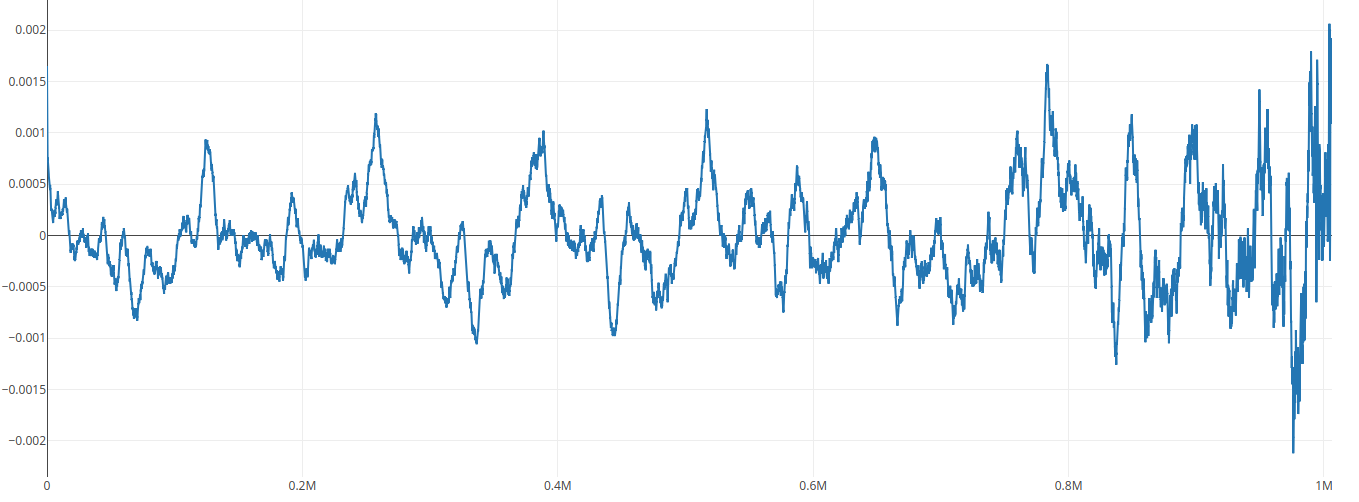
\includegraphics[width=.9\textwidth]{images/concatemer_mpm_10k.png}
}
\\
\subfloat[NSDF signal smoothed by 20k window\label{fig:acf_mpm20k}]{
	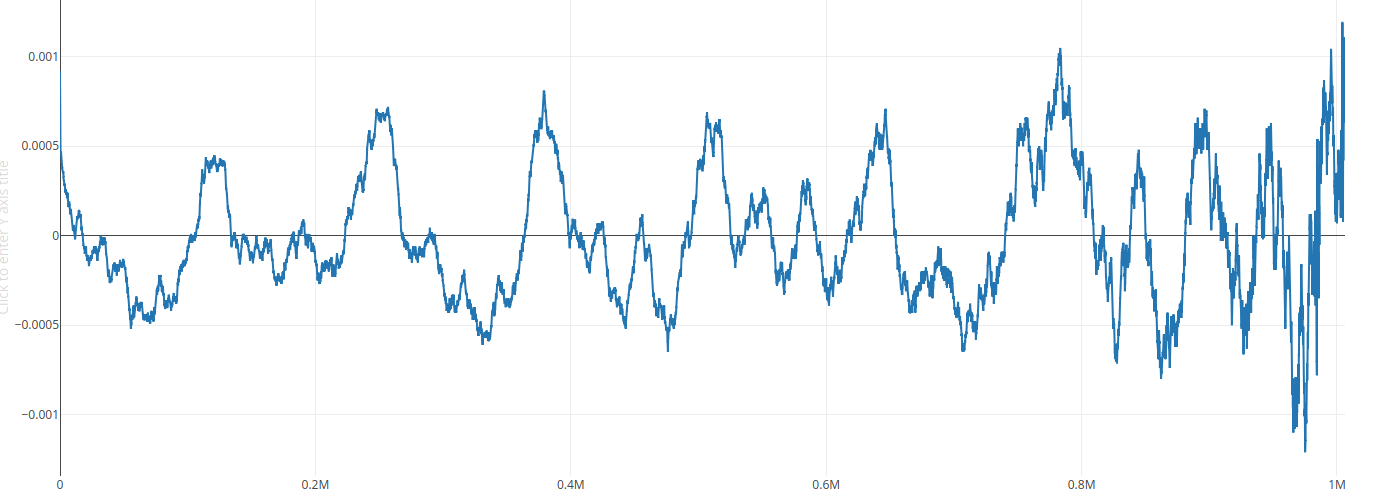
\includegraphics[width=.9\textwidth]{images/concatemer_mpm_20k.png}
}
\caption[NSDF signal processed by smoothing technique with different window size]{NSDF signal processed by smoothing technique with different window size values ($ws$): (\ref{fig:acf_mpm10k}) $ws=10,000$ (\ref{fig:acf_mpm20k}) $ws=20,000$.}
\label{fig:concat_acf_raw}
\end{figure}

Resembling the previous NKDF system, a smoothing step is required but with much larger window size. Figure~\ref{fig:concat_acf_raw} plots the NSDF of the 7-concatemer read with smooth window size of $10,000$ and $20,000$. Note that only the right side of the symmetric graph is presented here, corresponding to $n \in [0;L)$.
While the larger window sizes mean better de-noised result signals, it also reduces the specificity of the local maxima. As can be seen from the Figure~\ref{fig:acf_mpm20k}, the peaking regions are easier to spot but their blunt tips would challenge the peak picking algorithm in determining the exact value of coordinates. We apply the window size $10,000$ for the cases of raw signal as it returned clear spikes for easier monomer length evaluation. 
Similar to the NKDF signal, the tailing effect hinders the detection of peaks from the far ends. However, with the estimated monomer length, we can limit the list of candidates for the final peaks. 
\section{Discussion}
\begin{itemize}
    \item rolling circle amplification + barcode MinION sequencing: an assembly method using only Nanopore data for small genome (bacterial plasmid or viral genomes)
    \item read-by-read rapid processing can be adapted to a streaming pipeline
    \item study variation within sample if have sufficient long k-concatemer
    \item ...
\end{itemize}